\documentclass[11pt]{beamer} % Khai báo dùng gói beamer
\usetheme{Madrid} %Khai báo gói chủ đề trình chiếu (theme)
\usefonttheme{serif}
\usepackage[utf8]{vietnam}
\usepackage{hyperref}
\hypersetup{
	colorlinks=true,
	linkcolor=red,
	filecolor=magenta,      
	urlcolor=cyan,
}
\title[\textcolor{white}{Ôn thi THPT Quốc Gia 2016}]{\LARGE \textbf{PHÂN TÍCH ĐỀ THI THPT\\ QUỐC GIA 2016}}
\author[Tăng Lâm Tường Vinh (Môn Toán)]{} %Tên tác giả
\date{}
\usepackage{amsmath}
\usepackage{amssymb}
\usepackage{amsthm}
\usepackage{graphicx}
\usepackage{url}
\usepackage{color}
\usepackage{pgf,tikz}
\usepackage{mathrsfs}
\usetikzlibrary{arrows}
\usepackage{tkz-tab}

\newcommand{\parallelsum}{\mathbin{\!/\mkern-5mu/\!}}
\newcommand\Fontvi{\fontsize{9}{7.2}\selectfont}
\newcommand{\C}{\mbox{\textbf{C}}}
\newcommand\FontviTen{\fontsize{8.5}{7.2}\selectfont}
\newcommand{\cau}[2]{\begin{block}{}
		{\color{red}\textbf{Câu #1.}} #2
	\end{block}
}
\newcommand{\divColSeven}[2]{\begin{tabular}{cc}
		\begin{minipage}[c]{4.3cm} 
			#1
		\end{minipage}&
		\begin{minipage}[c]{6.9cm} 
			#2
		\end{minipage}
	\end{tabular}
}
\newcommand{\divColEight}[2]{\begin{tabular}{cc}
		\begin{minipage}[c]{5.3cm} 
			#1
		\end{minipage}&
		\begin{minipage}[c]{6.4cm} 
			#2
		\end{minipage}
	\end{tabular}
}

\begin{document}
\begin{frame}
\titlepage %in trang tiêu đề
\end{frame}
\begin{frame}{\textbf{\qquad Phân tích Đề thi THPT Quốc gia 2016}}~\\[-15pt]
\cau{1}{Khảo sát sự biến thiên và vẽ đồ thị của hàm số $y=\dfrac{3-2x}{x-1}$}\pause
\begin{itemize}
	\item Tập xác định $D=\mathbb{R} \backslash \left\{ 1 \right\}$
	\item Đạo hàm: $y'=\dfrac{-1}{(x-1)^2}<0,~\forall x\in D$
	\item Hsnb trên các khoảng $(-\infty;1)$, $(1;+\infty)$ và không có đạt cực trị.		
	\item $\lim\limits_{x\rightarrow -\infty} =-2;  \lim\limits_{x\rightarrow +\infty} =-2\Rightarrow y=-2$ là tiệm cận ngang.
	\item $\lim\limits_{x\rightarrow 1^-} =-\infty; \lim\limits_{x\rightarrow 1^+} =+\infty\Rightarrow x=1$ là tiệm cận đứng.		
	\item Bảng biến thiên
	\begin{center}
		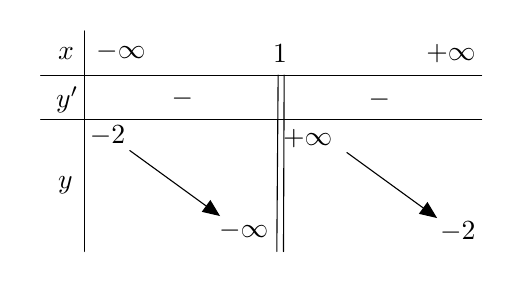
\begin{tikzpicture}[line cap=round,line join=round,>=triangle 45,x=0.28cm,y=0.28cm]
\clip(-4.5909616043916035,-6.210415814471959) rectangle (16.373084818128582,4.150427937698405);
\draw (-2.,4.)-- (-2.,-6.);
\draw (-4.,2.)-- (16.,2.);
\draw (-4.,0.)-- (16.,0.);
\draw (-3.6518207964463345,3.6960049661119854) node[anchor=north west] {$x$};
\draw (-3.7427053907636187,1.9086079445387356) node[anchor=north west] {$y'$};
\draw (-3.6518207964463345,-2.1811987997390396) node[anchor=north west] {$y$};
\draw (-1.9250135044179377,3.908069019518981) node[anchor=north west] {$-\infty$};
\draw (13.052713746568498,3.817184425201697) node[anchor=north west] {$+\infty$};
\draw (6.769612685268903,2.)-- (6.709022955724045,-6.);
\draw (7.042266468220754,2.)-- (7.011971603448327,-6.);
\draw (-2.2158980987352217,0.130326328648201815) node[anchor=north west] {$-2$};
\draw (3.649241613708817,-4.210954739491713) node[anchor=north west] {$-\infty$};
\draw (13.67684185338249,-4.210954739491713) node[anchor=north west] {$-2$};
\draw (6.554330521627751,-0.03026340089665411) node[anchor=north west] {$+\infty$};
\draw (1.498306214866428,1.7874284854490237) node[anchor=north west] {$-$};
\draw [->] (0.04415270578988331,-1.4238271804283404) -- (4.133959450067666,-4.392723928126282);
\draw [->] (9.889983756828988,-1.5147117747456242) -- (13.979790501106772,-4.4836085224435696);
\draw (6.103125660275486,3.817184425201697) node[anchor=north west] {$1$};
\draw (10.435021860222816,1.7571336206765957) node[anchor=north west] {$-$};
\end{tikzpicture}
	\end{center}
\end{itemize}
\end{frame}

\begin{frame}{\textbf{\qquad Phân tích Đề thi THPT Quốc gia 2016}}~\\[-20pt]
	\begin{itemize}
		\item Đồ thị\pause
		\begin{center}
			\documentclass[12pt]{article}
\usepackage{pstricks-add}
\usepackage{pst-text}
\pagestyle{empty}
\begin{document}
	\psset{xunit=1.0cm,yunit=1.0cm,algebraic=true,dimen=middle,dotstyle=o,dotsize=5pt 0,linewidth=0.8pt,arrowsize=3pt 2,arrowinset=0.25}
	\begin{pspicture*}(-8.808421624533308,-6.812028957659758)(8.513596421274286,3.9948420022619944)
	\psline[linewidth=1.2pt,linecolor=blue](-7.999999924372218,-2.1111111120447874)(-7.999999924372218,-2.1111111120447874)
	\psline[linewidth=1.2pt,linecolor=blue](-7.999999924372218,-2.1111111120447874)(-7.955499875482023,-2.111663225269843)
	\psline[linewidth=1.2pt,linecolor=blue](-7.955499875482023,-2.111663225269843)(-7.910999826591829,-2.112220852817867)
	\psline[linewidth=1.2pt,linecolor=blue](-7.910999826591829,-2.112220852817867)(-7.866499777701635,-2.112784077716316)
	\psline[linewidth=1.2pt,linecolor=blue](-7.866499777701635,-2.112784077716316)(-7.8219997288114405,-2.1133529846678796)
	\psline[linewidth=1.2pt,linecolor=blue](-7.8219997288114405,-2.1133529846678796)(-7.777499679921246,-2.113927660092945)
	\psline[linewidth=1.2pt,linecolor=blue](-7.777499679921246,-2.113927660092945)(-7.732999631031052,-2.1145081921733615)
	\psline[linewidth=1.2pt,linecolor=blue](-7.732999631031052,-2.1145081921733615)(-7.6884995821408575,-2.1150946708975495)
	\psline[linewidth=1.2pt,linecolor=blue](-7.6884995821408575,-2.1150946708975495)(-7.643999533250663,-2.1156871881070014)
	\psline[linewidth=1.2pt,linecolor=blue](-7.643999533250663,-2.1156871881070014)(-7.599499484360469,-2.1162858375442264)
	\psline[linewidth=1.2pt,linecolor=blue](-7.599499484360469,-2.1162858375442264)(-7.5549994354702745,-2.1168907149021954)
	\psline[linewidth=1.2pt,linecolor=blue](-7.5549994354702745,-2.1168907149021954)(-7.51049938658008,-2.1175019178753325)
	\psline[linewidth=1.2pt,linecolor=blue](-7.51049938658008,-2.1175019178753325)(-7.465999337689886,-2.1181195462121156)
	\psline[linewidth=1.2pt,linecolor=blue](-7.465999337689886,-2.1181195462121156)(-7.421499288799692,-2.1187437017693473)
	\psline[linewidth=1.2pt,linecolor=blue](-7.421499288799692,-2.1187437017693473)(-7.376999239909497,-2.1193744885681527)
	\psline[linewidth=1.2pt,linecolor=blue](-7.376999239909497,-2.1193744885681527)(-7.332499191019303,-2.1200120128517734)
	\psline[linewidth=1.2pt,linecolor=blue](-7.332499191019303,-2.1200120128517734)(-7.287999142129109,-2.120656383145222)
	\psline[linewidth=1.2pt,linecolor=blue](-7.287999142129109,-2.120656383145222)(-7.243499093238914,-2.121307710316869)
	\psline[linewidth=1.2pt,linecolor=blue](-7.243499093238914,-2.121307710316869)(-7.19899904434872,-2.1219661076420375)
	\psline[linewidth=1.2pt,linecolor=blue](-7.19899904434872,-2.1219661076420375)(-7.154498995458526,-2.122631690868676)
	\psline[linewidth=1.2pt,linecolor=blue](-7.154498995458526,-2.122631690868676)(-7.109998946568331,-2.123304578285197)
	\psline[linewidth=1.2pt,linecolor=blue](-7.109998946568331,-2.123304578285197)(-7.065498897678137,-2.123984890790559)
	\psline[linewidth=1.2pt,linecolor=blue](-7.065498897678137,-2.123984890790559)(-7.020998848787943,-2.1246727519666844)
	\psline[linewidth=1.2pt,linecolor=blue](-7.020998848787943,-2.1246727519666844)(-6.976498799897748,-2.125368288153296)
	\psline[linewidth=1.2pt,linecolor=blue](-6.976498799897748,-2.125368288153296)(-6.931998751007554,-2.126071628525279)
	\psline[linewidth=1.2pt,linecolor=blue](-6.931998751007554,-2.126071628525279)(-6.88749870211736,-2.126782905172657)
	\psline[linewidth=1.2pt,linecolor=blue](-6.88749870211736,-2.126782905172657)(-6.842998653227165,-2.1275022531832937)
	\psline[linewidth=1.2pt,linecolor=blue](-6.842998653227165,-2.1275022531832937)(-6.798498604336971,-2.1282298107284228)
	\psline[linewidth=1.2pt,linecolor=blue](-6.798498604336971,-2.1282298107284228)(-6.753998555446777,-2.128965719151128)
	\psline[linewidth=1.2pt,linecolor=blue](-6.753998555446777,-2.128965719151128)(-6.709498506556582,-2.12971012305788)
	\psline[linewidth=1.2pt,linecolor=blue](-6.709498506556582,-2.12971012305788)(-6.664998457666388,-2.1304631704132726)
	\psline[linewidth=1.2pt,linecolor=blue](-6.664998457666388,-2.1304631704132726)(-6.620498408776194,-2.1312250126380636)
	\psline[linewidth=1.2pt,linecolor=blue](-6.620498408776194,-2.1312250126380636)(-6.5759983598859995,-2.1319958047106877)
	\psline[linewidth=1.2pt,linecolor=blue](-6.5759983598859995,-2.1319958047106877)(-6.531498310995805,-2.132775705272352)
	\psline[linewidth=1.2pt,linecolor=blue](-6.531498310995805,-2.132775705272352)(-6.486998262105611,-2.1335648767358957)
	\psline[linewidth=1.2pt,linecolor=blue](-6.486998262105611,-2.1335648767358957)(-6.4424982132154165,-2.134363485398536)
	\psline[linewidth=1.2pt,linecolor=blue](-6.4424982132154165,-2.134363485398536)(-6.397998164325222,-2.135171701558703)
	\psline[linewidth=1.2pt,linecolor=blue](-6.397998164325222,-2.135171701558703)(-6.353498115435028,-2.1359896996371015)
	\psline[linewidth=1.2pt,linecolor=blue](-6.353498115435028,-2.1359896996371015)(-6.3089980665448335,-2.136817658302204)
	\psline[linewidth=1.2pt,linecolor=blue](-6.3089980665448335,-2.136817658302204)(-6.264498017654639,-2.137655760600352)
	\psline[linewidth=1.2pt,linecolor=blue](-6.264498017654639,-2.137655760600352)(-6.219997968764445,-2.138504194090671)
	\psline[linewidth=1.2pt,linecolor=blue](-6.219997968764445,-2.138504194090671)(-6.175497919874251,-2.1393631509850017)
	\psline[linewidth=1.2pt,linecolor=blue](-6.175497919874251,-2.1393631509850017)(-6.130997870984056,-2.1402328282930765)
	\psline[linewidth=1.2pt,linecolor=blue](-6.130997870984056,-2.1402328282930765)(-6.086497822093862,-2.1411134279731603)
	\psline[linewidth=1.2pt,linecolor=blue](-6.086497822093862,-2.1411134279731603)(-6.041997773203668,-2.1420051570884073)
	\psline[linewidth=1.2pt,linecolor=blue](-6.041997773203668,-2.1420051570884073)(-5.997497724313473,-2.142908227969179)
	\psline[linewidth=1.2pt,linecolor=blue](-5.997497724313473,-2.142908227969179)(-5.952997675423279,-2.1438228583816006)
	\psline[linewidth=1.2pt,linecolor=blue](-5.952997675423279,-2.1438228583816006)(-5.908497626533085,-2.1447492717026284)
	\psline[linewidth=1.2pt,linecolor=blue](-5.908497626533085,-2.1447492717026284)(-5.86399757764289,-2.1456876971019274)
	\psline[linewidth=1.2pt,linecolor=blue](-5.86399757764289,-2.1456876971019274)(-5.819497528752696,-2.146638369730871)
	\psline[linewidth=1.2pt,linecolor=blue](-5.819497528752696,-2.146638369730871)(-5.774997479862502,-2.1476015309189895)
	\psline[linewidth=1.2pt,linecolor=blue](-5.774997479862502,-2.1476015309189895)(-5.730497430972307,-2.148577428378208)
	\psline[linewidth=1.2pt,linecolor=blue](-5.730497430972307,-2.148577428378208)(-5.685997382082113,-2.149566316415246)
	\psline[linewidth=1.2pt,linecolor=blue](-5.685997382082113,-2.149566316415246)(-5.641497333191919,-2.1505684561525524)
	\psline[linewidth=1.2pt,linecolor=blue](-5.641497333191919,-2.1505684561525524)(-5.596997284301724,-2.1515841157581814)
	\psline[linewidth=1.2pt,linecolor=blue](-5.596997284301724,-2.1515841157581814)(-5.55249723541153,-2.152613570685039)
	\psline[linewidth=1.2pt,linecolor=blue](-5.55249723541153,-2.152613570685039)(-5.507997186521336,-2.1536571039199424)
	\psline[linewidth=1.2pt,linecolor=blue](-5.507997186521336,-2.1536571039199424)(-5.463497137631141,-2.154715006242967)
	\psline[linewidth=1.2pt,linecolor=blue](-5.463497137631141,-2.154715006242967)(-5.418997088740947,-2.155787576497584)
	\psline[linewidth=1.2pt,linecolor=blue](-5.418997088740947,-2.155787576497584)(-5.374497039850753,-2.1568751218721114)
	\psline[linewidth=1.2pt,linecolor=blue](-5.374497039850753,-2.1568751218721114)(-5.3299969909605585,-2.1579779581930345)
	\psline[linewidth=1.2pt,linecolor=blue](-5.3299969909605585,-2.1579779581930345)(-5.285496942070364,-2.1590964102307897)
	\psline[linewidth=1.2pt,linecolor=blue](-5.285496942070364,-2.1590964102307897)(-5.24099689318017,-2.160230812018629)
	\psline[linewidth=1.2pt,linecolor=blue](-5.24099689318017,-2.160230812018629)(-5.1964968442899755,-2.161381507185224)
	\psline[linewidth=1.2pt,linecolor=blue](-5.1964968442899755,-2.161381507185224)(-5.151996795399781,-2.1625488493017033)
	\psline[linewidth=1.2pt,linecolor=blue](-5.151996795399781,-2.1625488493017033)(-5.107496746509587,-2.163733202243865)
	\psline[linewidth=1.2pt,linecolor=blue](-5.107496746509587,-2.163733202243865)(-5.0629966976193925,-2.1649349405703364)
	\psline[linewidth=1.2pt,linecolor=blue](-5.0629966976193925,-2.1649349405703364)(-5.018496648729198,-2.1661544499175136)
	\psline[linewidth=1.2pt,linecolor=blue](-5.018496648729198,-2.1661544499175136)(-4.973996599839004,-2.1673921274121497)
	\psline[linewidth=1.2pt,linecolor=blue](-4.973996599839004,-2.1673921274121497)(-4.92949655094881,-2.1686483821025218)
	\psline[linewidth=1.2pt,linecolor=blue](-4.92949655094881,-2.1686483821025218)(-4.884996502058615,-2.1699236354091616)
	\psline[linewidth=1.2pt,linecolor=blue](-4.884996502058615,-2.1699236354091616)(-4.840496453168421,-2.17121832159619)
	\psline[linewidth=1.2pt,linecolor=blue](-4.840496453168421,-2.17121832159619)(-4.795996404278227,-2.1725328882643655)
	\psline[linewidth=1.2pt,linecolor=blue](-4.795996404278227,-2.1725328882643655)(-4.751496355388032,-2.1738677968670177)
	\psline[linewidth=1.2pt,linecolor=blue](-4.751496355388032,-2.1738677968670177)(-4.706996306497838,-2.175223523250125)
	\psline[linewidth=1.2pt,linecolor=blue](-4.706996306497838,-2.175223523250125)(-4.662496257607644,-2.1766005582178507)
	\psline[linewidth=1.2pt,linecolor=blue](-4.662496257607644,-2.1766005582178507)(-4.617996208717449,-2.1779994081249643)
	\psline[linewidth=1.2pt,linecolor=blue](-4.617996208717449,-2.1779994081249643)(-4.573496159827255,-2.1794205954976373)
	\psline[linewidth=1.2pt,linecolor=blue](-4.573496159827255,-2.1794205954976373)(-4.528996110937061,-2.1808646596842185)
	\psline[linewidth=1.2pt,linecolor=blue](-4.528996110937061,-2.1808646596842185)(-4.484496062046866,-2.1823321575376955)
	\psline[linewidth=1.2pt,linecolor=blue](-4.484496062046866,-2.1823321575376955)(-4.439996013156672,-2.183823664131645)
	\psline[linewidth=1.2pt,linecolor=blue](-4.439996013156672,-2.183823664131645)(-4.395495964266478,-2.1853397735116182)
	\psline[linewidth=1.2pt,linecolor=blue](-4.395495964266478,-2.1853397735116182)(-4.350995915376283,-2.186881099484016)
	\psline[linewidth=1.2pt,linecolor=blue](-4.350995915376283,-2.186881099484016)(-4.306495866486089,-2.188448276444657)
	\psline[linewidth=1.2pt,linecolor=blue](-4.306495866486089,-2.188448276444657)(-4.261995817595895,-2.190041960249387)
	\psline[linewidth=1.2pt,linecolor=blue](-4.261995817595895,-2.190041960249387)(-4.2174957687057,-2.1916628291292453)
	\psline[linewidth=1.2pt,linecolor=blue](-4.2174957687057,-2.1916628291292453)(-4.172995719815506,-2.1933115846528604)
	\psline[linewidth=1.2pt,linecolor=blue](-4.172995719815506,-2.1933115846528604)(-4.128495670925312,-2.1949889527389566)
	\psline[linewidth=1.2pt,linecolor=blue](-4.128495670925312,-2.1949889527389566)(-4.0839956220351175,-2.19669568472203)
	\psline[linewidth=1.2pt,linecolor=blue](-4.0839956220351175,-2.19669568472203)(-4.039495573144923,-2.1984325584744875)
	\psline[linewidth=1.2pt,linecolor=blue](-4.039495573144923,-2.1984325584744875)(-3.994995524254729,-2.200200379588769)
	\psline[linewidth=1.2pt,linecolor=blue](-3.994995524254729,-2.200200379588769)(-3.9504954753645345,-2.201999982623227)
	\psline[linewidth=1.2pt,linecolor=blue](-3.9504954753645345,-2.201999982623227)(-3.90599542647434,-2.2038322324158064)
	\psline[linewidth=1.2pt,linecolor=blue](-3.90599542647434,-2.2038322324158064)(-3.861495377584146,-2.2056980254698786)
	\psline[linewidth=1.2pt,linecolor=blue](-3.861495377584146,-2.2056980254698786)(-3.8169953286939515,-2.207598291416889)
	\psline[linewidth=1.2pt,linecolor=blue](-3.8169953286939515,-2.207598291416889)(-3.772495279803757,-2.2095339945608328)
	\psline[linewidth=1.2pt,linecolor=blue](-3.772495279803757,-2.2095339945608328)(-3.727995230913563,-2.21150613550995)
	\psline[linewidth=1.2pt,linecolor=blue](-3.727995230913563,-2.21150613550995)(-3.6834951820233686,-2.213515752901443)
	\psline[linewidth=1.2pt,linecolor=blue](-3.6834951820233686,-2.213515752901443)(-3.6389951331331742,-2.2155639252254615)
	\psline[linewidth=1.2pt,linecolor=blue](-3.6389951331331742,-2.2155639252254615)(-3.59449508424298,-2.217651772755083)
	\psline[linewidth=1.2pt,linecolor=blue](-3.59449508424298,-2.217651772755083)(-3.5499950353527856,-2.2197804595895487)
	\psline[linewidth=1.2pt,linecolor=blue](-3.5499950353527856,-2.2197804595895487)(-3.5054949864625913,-2.2219511958185825)
	\psline[linewidth=1.2pt,linecolor=blue](-3.5054949864625913,-2.2219511958185825)(-3.460994937572397,-2.2241652398162515)
	\psline[linewidth=1.2pt,linecolor=blue](-3.460994937572397,-2.2241652398162515)(-3.4164948886822026,-2.2264239006735003)
	\psline[linewidth=1.2pt,linecolor=blue](-3.4164948886822026,-2.2264239006735003)(-3.3719948397920083,-2.2287285407792417)
	\psline[linewidth=1.2pt,linecolor=blue](-3.3719948397920083,-2.2287285407792417)(-3.327494790901814,-2.2310805785606984)
	\psline[linewidth=1.2pt,linecolor=blue](-3.327494790901814,-2.2310805785606984)(-3.2829947420116197,-2.233481491394576)
	\psline[linewidth=1.2pt,linecolor=blue](-3.2829947420116197,-2.233481491394576)(-3.2384946931214253,-2.235932818701621)
	\psline[linewidth=1.2pt,linecolor=blue](-3.2384946931214253,-2.235932818701621)(-3.193994644231231,-2.2384361652381894)
	\psline[linewidth=1.2pt,linecolor=blue](-3.193994644231231,-2.2384361652381894)(-3.1494945953410367,-2.2409932045996106)
	\psline[linewidth=1.2pt,linecolor=blue](-3.1494945953410367,-2.2409932045996106)(-3.1049945464508424,-2.2436056829514173)
	\psline[linewidth=1.2pt,linecolor=blue](-3.1049945464508424,-2.2436056829514173)(-3.060494497560648,-2.24627542300593)
	\psline[linewidth=1.2pt,linecolor=blue](-3.060494497560648,-2.24627542300593)(-3.0159944486704537,-2.249004328263218)
	\psline[linewidth=1.2pt,linecolor=blue](-3.0159944486704537,-2.249004328263218)(-2.9714943997802594,-2.2517943875371773)
	\psline[linewidth=1.2pt,linecolor=blue](-2.9714943997802594,-2.2517943875371773)(-2.926994350890065,-2.2546476797893398)
	\psline[linewidth=1.2pt,linecolor=blue](-2.926994350890065,-2.2546476797893398)(-2.882494301999871,-2.2575663792951093)
	\psline[linewidth=1.2pt,linecolor=blue](-2.882494301999871,-2.2575663792951093)(-2.8379942531096765,-2.260552761169396)
	\psline[linewidth=1.2pt,linecolor=blue](-2.8379942531096765,-2.260552761169396)(-2.793494204219482,-2.263609207281167)
	\psline[linewidth=1.2pt,linecolor=blue](-2.793494204219482,-2.263609207281167)(-2.748994155329288,-2.266738212589229)
	\psline[linewidth=1.2pt,linecolor=blue](-2.748994155329288,-2.266738212589229)(-2.7044941064390935,-2.269942391934655)
	\psline[linewidth=1.2pt,linecolor=blue](-2.7044941064390935,-2.269942391934655)(-2.659994057548899,-2.273224487328731)
	\psline[linewidth=1.2pt,linecolor=blue](-2.659994057548899,-2.273224487328731)(-2.615494008658705,-2.2765873757791084)
	\psline[linewidth=1.2pt,linecolor=blue](-2.615494008658705,-2.2765873757791084)(-2.5709939597685105,-2.2800340777011074)
	\psline[linewidth=1.2pt,linecolor=blue](-2.5709939597685105,-2.2800340777011074)(-2.526493910878316,-2.2835677659658677)
	\psline[linewidth=1.2pt,linecolor=blue](-2.526493910878316,-2.2835677659658677)(-2.481993861988122,-2.287191775642312)
	\psline[linewidth=1.2pt,linecolor=blue](-2.481993861988122,-2.287191775642312)(-2.4374938130979276,-2.290909614495795)
	\psline[linewidth=1.2pt,linecolor=blue](-2.4374938130979276,-2.290909614495795)(-2.3929937642077332,-2.2947249743129134)
	\psline[linewidth=1.2pt,linecolor=blue](-2.3929937642077332,-2.2947249743129134)(-2.348493715317539,-2.2986417431293193)
	\psline[linewidth=1.2pt,linecolor=blue](-2.348493715317539,-2.2986417431293193)(-2.3039936664273446,-2.3026640184456872)
	\psline[linewidth=1.2pt,linecolor=blue](-2.3039936664273446,-2.3026640184456872)(-2.2594936175371503,-2.306796121526261)
	\psline[linewidth=1.2pt,linecolor=blue](-2.2594936175371503,-2.306796121526261)(-2.214993568646956,-2.3110426128848696)
	\psline[linewidth=1.2pt,linecolor=blue](-2.214993568646956,-2.3110426128848696)(-2.1704935197567616,-2.3154083090750865)
	\psline[linewidth=1.2pt,linecolor=blue](-2.1704935197567616,-2.3154083090750865)(-2.1259934708665673,-2.3198983009144887)
	\psline[linewidth=1.2pt,linecolor=blue](-2.1259934708665673,-2.3198983009144887)(-2.081493421976373,-2.3245179732879753)
	\psline[linewidth=1.2pt,linecolor=blue](-2.081493421976373,-2.3245179732879753)(-2.0369933730861787,-2.329273026692121)
	\psline[linewidth=1.2pt,linecolor=blue](-2.0369933730861787,-2.329273026692121)(-1.9924933241959843,-2.334169500701786)
	\psline[linewidth=1.2pt,linecolor=blue](-1.9924933241959843,-2.334169500701786)(-1.94799327530579,-2.339213799562101)
	\psline[linewidth=1.2pt,linecolor=blue](-1.94799327530579,-2.339213799562101)(-1.9034932264155957,-2.3444127201338487)
	\psline[linewidth=1.2pt,linecolor=blue](-1.9034932264155957,-2.3444127201338487)(-1.8589931775254014,-2.349773482448653)
	\psline[linewidth=1.2pt,linecolor=blue](-1.8589931775254014,-2.349773482448653)(-1.814493128635207,-2.355303763162824)
	\psline[linewidth=1.2pt,linecolor=blue](-1.814493128635207,-2.355303763162824)(-1.7699930797450127,-2.361011732235827)
	\psline[linewidth=1.2pt,linecolor=blue](-1.7699930797450127,-2.361011732235827)(-1.7254930308548184,-2.3669060932019197)
	\psline[linewidth=1.2pt,linecolor=blue](-1.7254930308548184,-2.3669060932019197)(-1.680992981964624,-2.3729961274524496)
	\psline[linewidth=1.2pt,linecolor=blue](-1.680992981964624,-2.3729961274524496)(-1.6364929330744298,-2.3792917430026614)
	\psline[linewidth=1.2pt,linecolor=blue](-1.6364929330744298,-2.3792917430026614)(-1.5919928841842355,-2.3858035282819556)
	\psline[linewidth=1.2pt,linecolor=blue](-1.5919928841842355,-2.3858035282819556)(-1.5474928352940411,-2.3925428115618534)
	\psline[linewidth=1.2pt,linecolor=blue](-1.5474928352940411,-2.3925428115618534)(-1.5029927864038468,-2.3995217267232887)
	\psline[linewidth=1.2pt,linecolor=blue](-1.5029927864038468,-2.3995217267232887)(-1.4584927375136525,-2.406753286166438)
	\psline[linewidth=1.2pt,linecolor=blue](-1.4584927375136525,-2.406753286166438)(-1.4139926886234582,-2.414251461784764)
	\psline[linewidth=1.2pt,linecolor=blue](-1.4139926886234582,-2.414251461784764)(-1.3694926397332639,-2.422031275063412)
	\psline[linewidth=1.2pt,linecolor=blue](-1.3694926397332639,-2.422031275063412)(-1.3249925908430695,-2.430108897524438)
	\psline[linewidth=1.2pt,linecolor=blue](-1.3249925908430695,-2.430108897524438)(-1.2804925419528752,-2.4385017629321695)
	\psline[linewidth=1.2pt,linecolor=blue](-1.2804925419528752,-2.4385017629321695)(-1.2359924930626809,-2.4472286928970326)
	\psline[linewidth=1.2pt,linecolor=blue](-1.2359924930626809,-2.4472286928970326)(-1.1914924441724866,-2.4563100377823126)
	\psline[linewidth=1.2pt,linecolor=blue](-1.1914924441724866,-2.4563100377823126)(-1.1469923952822922,-2.4657678351340957)
	\psline[linewidth=1.2pt,linecolor=blue](-1.1469923952822922,-2.4657678351340957)(-1.102492346392098,-2.475625988230593)
	\psline[linewidth=1.2pt,linecolor=blue](-1.102492346392098,-2.475625988230593)(-1.0579922975019036,-2.485910467796139)
	\psline[linewidth=1.2pt,linecolor=blue](-1.0579922975019036,-2.485910467796139)(-1.0134922486117093,-2.496649540463587)
	\psline[linewidth=1.2pt,linecolor=blue](-1.0134922486117093,-2.496649540463587)(-0.9689921997215151,-2.5078740282167877)
	\psline[linewidth=1.2pt,linecolor=blue](-0.9689921997215151,-2.5078740282167877)(-0.9244921508313209,-2.5196176038276024)
	\psline[linewidth=1.2pt,linecolor=blue](-0.9244921508313209,-2.5196176038276024)(-0.8799921019411266,-2.5319171282514863)
	\psline[linewidth=1.2pt,linecolor=blue](-0.8799921019411266,-2.5319171282514863)(-0.8354920530509324,-2.544813037102401)
	\psline[linewidth=1.2pt,linecolor=blue](-0.8354920530509324,-2.544813037102401)(-0.7909920041607382,-2.5583497847432333)
	\psline[linewidth=1.2pt,linecolor=blue](-0.7909920041607382,-2.5583497847432333)(-0.746491955270544,-2.5725763562678954)
	\psline[linewidth=1.2pt,linecolor=blue](-0.746491955270544,-2.5725763562678954)(-0.7019919063803498,-2.5875468598007108)
	\psline[linewidth=1.2pt,linecolor=blue](-0.7019919063803498,-2.5875468598007108)(-0.6574918574901556,-2.603321214207497)
	\psline[linewidth=1.2pt,linecolor=blue](-0.6574918574901556,-2.603321214207497)(-0.6129918085999614,-2.619965950644211)
	\psline[linewidth=1.2pt,linecolor=blue](-0.6129918085999614,-2.619965950644211)(-0.5684917597097672,-2.6375551505511505)
	\psline[linewidth=1.2pt,linecolor=blue](-0.5684917597097672,-2.6375551505511505)(-0.523991710819573,-2.6561715479818586)
	\psline[linewidth=1.2pt,linecolor=blue](-0.523991710819573,-2.6561715479818586)(-0.47949166192937875,-2.6759078308666626)
	\psline[linewidth=1.2pt,linecolor=blue](-0.47949166192937875,-2.6759078308666626)(-0.43499161303918454,-2.6968681843945337)
	\psline[linewidth=1.2pt,linecolor=blue](-0.43499161303918454,-2.6968681843945337)(-0.39049156414899033,-2.7191701307530196)
	\psline[linewidth=1.2pt,linecolor=blue](-0.39049156414899033,-2.7191701307530196)(-0.3459915152587961,-2.742946733811861)
	\psline[linewidth=1.2pt,linecolor=blue](-0.3459915152587961,-2.742946733811861)(-0.3014914663686019,-2.7683492560963017)
	\psline[linewidth=1.2pt,linecolor=blue](-0.3014914663686019,-2.7683492560963017)(-0.2569914174784077,-2.7955503801339026)
	\psline[linewidth=1.2pt,linecolor=blue](-0.2569914174784077,-2.7955503801339026)(-0.2124913685882135,-2.824748139167678)
	\psline[linewidth=1.2pt,linecolor=blue](-0.2124913685882135,-2.824748139167678)(-0.16799131969801928,-2.856170746421769)
	\psline[linewidth=1.2pt,linecolor=blue](-0.16799131969801928,-2.856170746421769)(-0.12349127080782506,-2.890082572053247)
	\psline[linewidth=1.2pt,linecolor=blue](-0.12349127080782506,-2.890082572053247)(-0.07899122191763083,-2.926791599122332)
	\psline[linewidth=1.2pt,linecolor=blue](-0.07899122191763083,-2.926791599122332)(-0.03449117302743661,-2.9666588039349837)
	\psline[linewidth=1.2pt,linecolor=blue](-0.03449117302743661,-2.9666588039349837)(0.010008875862757616,-3.0101100662609275)
	\psline[linewidth=1.2pt,linecolor=blue](0.010008875862757616,-3.0101100662609275)(0.05450892475295184,-3.057651442916803)
	\psline[linewidth=1.2pt,linecolor=blue](0.05450892475295184,-3.057651442916803)(0.09900897364314606,-3.1098889675333257)
	\psline[linewidth=1.2pt,linecolor=blue](0.09900897364314606,-3.1098889675333257)(0.1435090225333403,-3.1675546226509157)
	\psline[linewidth=1.2pt,linecolor=blue](0.1435090225333403,-3.1675546226509157)(0.1880090714235345,-3.2315408520057494)
	\psline[linewidth=1.2pt,linecolor=blue](0.1880090714235345,-3.2315408520057494)(0.23250912031372872,-3.3029470792001754)
	\psline[linewidth=1.2pt,linecolor=blue](0.23250912031372872,-3.3029470792001754)(0.27700916920392293,-3.38314340570393)
	\psline[linewidth=1.2pt,linecolor=blue](0.27700916920392293,-3.38314340570393)(0.32150921809411714,-3.4738593753492073)
	\psline[linewidth=1.2pt,linecolor=blue](0.32150921809411714,-3.4738593753492073)(0.36600926698431135,-3.5773101213062275)
	\psline[linewidth=1.2pt,linecolor=blue](0.36600926698431135,-3.5773101213062275)(0.41050931587450556,-3.6963796492958894)
	\psline[linewidth=1.2pt,linecolor=blue](0.41050931587450556,-3.6963796492958894)(0.4550093647646998,-3.834893914403225)
	\psline[linewidth=1.2pt,linecolor=blue](0.4550093647646998,-3.834893914403225)(0.499509413654894,-3.9980395781319737)
	\psline[linewidth=1.2pt,linecolor=blue](0.499509413654894,-3.9980395781319737)(0.5440094625450882,-4.193027964092083)
	\psline[linewidth=1.2pt,linecolor=blue](0.5440094625450882,-4.193027964092083)(0.5885095114352824,-4.430189828902264)
	\psline[linewidth=1.2pt,linecolor=blue](0.5885095114352824,-4.430189828902264)(0.6330095603254766,-4.724866622920423)
	\psline[linewidth=1.2pt,linecolor=blue](0.6330095603254766,-4.724866622920423)(0.6775096092156708,-5.100867587303607)
	\psline[linewidth=1.2pt,linecolor=blue](0.6775096092156708,-5.100867587303607)(0.722009658105865,-5.597247275521617)
	\psline[linewidth=1.2pt,linecolor=blue](0.722009658105865,-5.597247275521617)(0.7665097069960592,-6.282833290988771)
	\psline[linewidth=1.2pt,linecolor=blue](0.7665097069960592,-6.282833290988771)(0.8110097558862535,-7.2912784185734765)
	\psline[linewidth=1.2pt,linecolor=blue](0.8110097558862535,-7.2912784185734765)(0.8555098047764477,-8.920884828571378)
	\psline[linewidth=1.2pt,linecolor=blue](1.1000001357655669,7.999986423461745)(1.1000001357655669,7.999986423461745)
	\psline[linewidth=1.2pt,linecolor=blue](1.1000001357655669,7.999986423461745)(1.1345001715757732,5.43493475349681)
	\psline[linewidth=1.2pt,linecolor=blue](1.1345001715757732,5.43493475349681)(1.1690002073859795,3.9171525021629128)
	\psline[linewidth=1.2pt,linecolor=blue](1.1690002073859795,3.9171525021629128)(1.2035002431961859,2.913999041445581)
	\psline[linewidth=1.2pt,linecolor=blue](1.2035002431961859,2.913999041445581)(1.2380002790063922,2.2016757466622217)
	\psline[linewidth=1.2pt,linecolor=blue](1.2380002790063922,2.2016757466622217)(1.2725003148165985,1.6697205310497794)
	\psline[linewidth=1.2pt,linecolor=blue](1.2725003148165985,1.6697205310497794)(1.3070003506268049,1.2573252700144892)
	\psline[linewidth=1.2pt,linecolor=blue](1.3070003506268049,1.2573252700144892)(1.3415003864370112,0.9282543731014116)
	\psline[linewidth=1.2pt,linecolor=blue](1.3415003864370112,0.9282543731014116)(1.3760004222472175,0.6595714813918675)
	\psline[linewidth=1.2pt,linecolor=blue](1.3760004222472175,0.6595714813918675)(1.4105004580574239,0.4360508749057536)
	\psline[linewidth=1.2pt,linecolor=blue](1.4105004580574239,0.4360508749057536)(1.4450004938676302,0.24718851727265706)
	\psline[linewidth=1.2pt,linecolor=blue](1.4450004938676302,0.24718851727265706)(1.4795005296778365,0.08550343139740231)
	\psline[linewidth=1.2pt,linecolor=blue](1.4795005296778365,0.08550343139740231)(1.5140005654880428,-0.05447684857992065)
	\psline[linewidth=1.2pt,linecolor=blue](1.5140005654880428,-0.05447684857992065)(1.5485006012982492,-0.17684794212969987)
	\psline[linewidth=1.2pt,linecolor=blue](1.5485006012982492,-0.17684794212969987)(1.5830006371084555,-0.2847360082490439)
	\psline[linewidth=1.2pt,linecolor=blue](1.5830006371084555,-0.2847360082490439)(1.6175006729186618,-0.3805685663896895)
	\psline[linewidth=1.2pt,linecolor=blue](1.6175006729186618,-0.3805685663896895)(1.6520007087288682,-0.46625933589921004)
	\psline[linewidth=1.2pt,linecolor=blue](1.6520007087288682,-0.46625933589921004)(1.6865007445390745,-0.5433373409210023)
	\psline[linewidth=1.2pt,linecolor=blue](1.6865007445390745,-0.5433373409210023)(1.7210007803492808,-0.6130389491179731)
	\psline[linewidth=1.2pt,linecolor=blue](1.7210007803492808,-0.6130389491179731)(1.7555008161594872,-0.6763746926397777)
	\psline[linewidth=1.2pt,linecolor=blue](1.7555008161594872,-0.6763746926397777)(1.7900008519696935,-0.7341785803056797)
	\psline[linewidth=1.2pt,linecolor=blue](1.7900008519696935,-0.7341785803056797)(1.8245008877798998,-0.7871450294096596)
	\psline[linewidth=1.2pt,linecolor=blue](1.8245008877798998,-0.7871450294096596)(1.8590009235901062,-0.8358568977777082)
	\psline[linewidth=1.2pt,linecolor=blue](1.8590009235901062,-0.8358568977777082)(1.8935009594003125,-0.8808070215490691)
	\psline[linewidth=1.2pt,linecolor=blue](1.8935009594003125,-0.8808070215490691)(1.9280009952105188,-0.9224149487327349)
	\psline[linewidth=1.2pt,linecolor=blue](1.9280009952105188,-0.9224149487327349)(1.9625010310207252,-0.9610400739628222)
	\psline[linewidth=1.2pt,linecolor=blue](1.9625010310207252,-0.9610400739628222)(1.9970010668309315,-0.996992046178445)
	\psline[linewidth=1.2pt,linecolor=blue](1.9970010668309315,-0.996992046178445)(2.031501102641138,-1.0305390877047826)
	\psline[linewidth=1.2pt,linecolor=blue](2.031501102641138,-1.0305390877047826)(2.066001138451344,-1.0619146979028828)
	\psline[linewidth=1.2pt,linecolor=blue](2.066001138451344,-1.0619146979028828)(2.1005011742615505,-1.0913230958876423)
	\psline[linewidth=1.2pt,linecolor=blue](2.1005011742615505,-1.0913230958876423)(2.135001210071757,-1.1189436706091458)
	\psline[linewidth=1.2pt,linecolor=blue](2.135001210071757,-1.1189436706091458)(2.169501245881963,-1.1449346432753358)
	\psline[linewidth=1.2pt,linecolor=blue](2.169501245881963,-1.1449346432753358)(2.2040012816921695,-1.1694361001056865)
	\psline[linewidth=1.2pt,linecolor=blue](2.2040012816921695,-1.1694361001056865)(2.238501317502376,-1.1925725181975175)
	\psline[linewidth=1.2pt,linecolor=blue](2.238501317502376,-1.1925725181975175)(2.273001353312582,-1.2144548806662168)
	\psline[linewidth=1.2pt,linecolor=blue](2.273001353312582,-1.2144548806662168)(2.3075013891227885,-1.2351824569219718)
	\psline[linewidth=1.2pt,linecolor=blue](2.3075013891227885,-1.2351824569219718)(2.342001424932995,-1.254844308343466)
	\psline[linewidth=1.2pt,linecolor=blue](2.342001424932995,-1.254844308343466)(2.376501460743201,-1.2735205675262562)
	\psline[linewidth=1.2pt,linecolor=blue](2.376501460743201,-1.2735205675262562)(2.4110014965534075,-1.2912835298597083)
	\psline[linewidth=1.2pt,linecolor=blue](2.4110014965534075,-1.2912835298597083)(2.445501532363614,-1.308198588786794)
	\psline[linewidth=1.2pt,linecolor=blue](2.445501532363614,-1.308198588786794)(2.48000156817382,-1.3243250402539073)
	\psline[linewidth=1.2pt,linecolor=blue](2.48000156817382,-1.3243250402539073)(2.5145016039840264,-1.33971677720947)
	\psline[linewidth=1.2pt,linecolor=blue](2.5145016039840264,-1.33971677720947)(2.5490016397942328,-1.3544228912934924)
	\psline[linewidth=1.2pt,linecolor=blue](2.5490016397942328,-1.3544228912934924)(2.583501675604439,-1.3684881958724233)
	\psline[linewidth=1.2pt,linecolor=blue](2.583501675604439,-1.3684881958724233)(2.6180017114146454,-1.3819536821591594)
	\psline[linewidth=1.2pt,linecolor=blue](2.6180017114146454,-1.3819536821591594)(2.6525017472248518,-1.3948569181972958)
	\psline[linewidth=1.2pt,linecolor=blue](2.6525017472248518,-1.3948569181972958)(2.687001783035058,-1.4072323988888051)
	\psline[linewidth=1.2pt,linecolor=blue](2.687001783035058,-1.4072323988888051)(2.7215018188452644,-1.4191118539329965)
	\psline[linewidth=1.2pt,linecolor=blue](2.7215018188452644,-1.4191118539329965)(2.7560018546554708,-1.4305245194651568)
	\psline[linewidth=1.2pt,linecolor=blue](2.7560018546554708,-1.4305245194651568)(2.790501890465677,-1.4414973782910008)
	\psline[linewidth=1.2pt,linecolor=blue](2.790501890465677,-1.4414973782910008)(2.8250019262758834,-1.452055372872614)
	\psline[linewidth=1.2pt,linecolor=blue](2.8250019262758834,-1.452055372872614)(2.8595019620860898,-1.4622215946047479)
	\psline[linewidth=1.2pt,linecolor=blue](2.8595019620860898,-1.4622215946047479)(2.894001997896296,-1.4720174524046337)
	\psline[linewidth=1.2pt,linecolor=blue](2.894001997896296,-1.4720174524046337)(2.9285020337065024,-1.4814628232058222)
	\psline[linewidth=1.2pt,linecolor=blue](2.9285020337065024,-1.4814628232058222)(2.9630020695167087,-1.4905761865823197)
	\psline[linewidth=1.2pt,linecolor=blue](2.9630020695167087,-1.4905761865823197)(2.997502105326915,-1.4993747454216886)
	\psline[linewidth=1.2pt,linecolor=blue](2.997502105326915,-1.4993747454216886)(3.0320021411371214,-1.5078745343051687)
	\psline[linewidth=1.2pt,linecolor=blue](3.0320021411371214,-1.5078745343051687)(3.0665021769473277,-1.5160905170314327)
	\psline[linewidth=1.2pt,linecolor=blue](3.0665021769473277,-1.5160905170314327)(3.101002212757534,-1.5240366745318583)
	\psline[linewidth=1.2pt,linecolor=blue](3.101002212757534,-1.5240366745318583)(3.1355022485677404,-1.531726084263929)
	\psline[linewidth=1.2pt,linecolor=blue](3.1355022485677404,-1.531726084263929)(3.1700022843779467,-1.5391709920311627)
	\psline[linewidth=1.2pt,linecolor=blue](3.1700022843779467,-1.5391709920311627)(3.204502320188153,-1.546382877059231)
	\psline[linewidth=1.2pt,linecolor=blue](3.204502320188153,-1.546382877059231)(3.2390023559983594,-1.5533725110556638)
	\psline[linewidth=1.2pt,linecolor=blue](3.2390023559983594,-1.5533725110556638)(3.2735023918085657,-1.5601500118922231)
	\psline[linewidth=1.2pt,linecolor=blue](3.2735023918085657,-1.5601500118922231)(3.308002427618772,-1.5667248924726103)
	\psline[linewidth=1.2pt,linecolor=blue](3.308002427618772,-1.5667248924726103)(3.3425024634289784,-1.5731061052818744)
	\psline[linewidth=1.2pt,linecolor=blue](3.3425024634289784,-1.5731061052818744)(3.3770024992391847,-1.5793020830562554)
	\psline[linewidth=1.2pt,linecolor=blue](3.3770024992391847,-1.5793020830562554)(3.411502535049391,-1.5853207759619798)
	\psline[linewidth=1.2pt,linecolor=blue](3.411502535049391,-1.5853207759619798)(3.4460025708595974,-1.5911696856276931)
	\psline[linewidth=1.2pt,linecolor=blue](3.4460025708595974,-1.5911696856276931)(3.4805026066698037,-1.596855896336852)
	\psline[linewidth=1.2pt,linecolor=blue](3.4805026066698037,-1.596855896336852)(3.51500264248001,-1.6023861036527924)
	\psline[linewidth=1.2pt,linecolor=blue](3.51500264248001,-1.6023861036527924)(3.5495026782902164,-1.6077666407196582)
	\psline[linewidth=1.2pt,linecolor=blue](3.5495026782902164,-1.6077666407196582)(3.5840027141004227,-1.6130035024564078)
	\psline[linewidth=1.2pt,linecolor=blue](3.5840027141004227,-1.6130035024564078)(3.618502749910629,-1.6181023678382118)
	\psline[linewidth=1.2pt,linecolor=blue](3.618502749910629,-1.6181023678382118)(3.6530027857208354,-1.6230686204393507)
	\psline[linewidth=1.2pt,linecolor=blue](3.6530027857208354,-1.6230686204393507)(3.6875028215310417,-1.6279073673938282)
	\psline[linewidth=1.2pt,linecolor=blue](3.6875028215310417,-1.6279073673938282)(3.722002857341248,-1.632623456914089)
	\psline[linewidth=1.2pt,linecolor=blue](3.722002857341248,-1.632623456914089)(3.7565028931514544,-1.6372214944941632)
	\psline[linewidth=1.2pt,linecolor=blue](3.7565028931514544,-1.6372214944941632)(3.7910029289616607,-1.6417058579110733)
	\psline[linewidth=1.2pt,linecolor=blue](3.7910029289616607,-1.6417058579110733)(3.825502964771867,-1.6460807111272167)
	\psline[linewidth=1.2pt,linecolor=blue](3.825502964771867,-1.6460807111272167)(3.8600030005820734,-1.6503500171865282)
	\psline[linewidth=1.2pt,linecolor=blue](3.8600030005820734,-1.6503500171865282)(3.8945030363922797,-1.6545175501883722)
	\psline[linewidth=1.2pt,linecolor=blue](3.8945030363922797,-1.6545175501883722)(3.929003072202486,-1.6585869064152117)
	\psline[linewidth=1.2pt,linecolor=blue](3.929003072202486,-1.6585869064152117)(3.9635031080126923,-1.6625615146830084)
	\psline[linewidth=1.2pt,linecolor=blue](3.9635031080126923,-1.6625615146830084)(3.9980031438228987,-1.6664446459769713)
	\psline[linewidth=1.2pt,linecolor=blue](3.9980031438228987,-1.6664446459769713)(4.032503179633105,-1.6702394224295627)
	\psline[linewidth=1.2pt,linecolor=blue](4.032503179633105,-1.6702394224295627)(4.067003215443311,-1.6739488256925554)
	\psline[linewidth=1.2pt,linecolor=blue](4.067003215443311,-1.6739488256925554)(4.101503251253517,-1.6775757047503221)
	\psline[linewidth=1.2pt,linecolor=blue](4.101503251253517,-1.6775757047503221)(4.136003287063723,-1.6811227832173887)
	\psline[linewidth=1.2pt,linecolor=blue](4.136003287063723,-1.6811227832173887)(4.1705033228739286,-1.6845926661595352)
	\psline[linewidth=1.2pt,linecolor=blue](4.1705033228739286,-1.6845926661595352)(4.205003358684134,-1.6879878464743432)
	\psline[linewidth=1.2pt,linecolor=blue](4.205003358684134,-1.6879878464743432)(4.23950339449434,-1.6913107108640362)
	\psline[linewidth=1.2pt,linecolor=blue](4.23950339449434,-1.6913107108640362)(4.274003430304546,-1.6945635454306838)
	\psline[linewidth=1.2pt,linecolor=blue](4.274003430304546,-1.6945635454306838)(4.308503466114752,-1.6977485409213362)
	\psline[linewidth=1.2pt,linecolor=blue](4.308503466114752,-1.6977485409213362)(4.343003501924958,-1.7008677976483773)
	\psline[linewidth=1.2pt,linecolor=blue](4.343003501924958,-1.7008677976483773)(4.377503537735164,-1.7039233301083188)
	\psline[linewidth=1.2pt,linecolor=blue](4.377503537735164,-1.7039233301083188)(4.41200357354537,-1.7069170713203818)
	\psline[linewidth=1.2pt,linecolor=blue](4.41200357354537,-1.7069170713203818)(4.446503609355576,-1.7098508769044989)
	\psline[linewidth=1.2pt,linecolor=blue](4.446503609355576,-1.7098508769044989)(4.4810036451657815,-1.7127265289168132)
	\psline[linewidth=1.2pt,linecolor=blue](4.4810036451657815,-1.7127265289168132)(4.515503680975987,-1.7155457394593379)
	\psline[linewidth=1.2pt,linecolor=blue](4.515503680975987,-1.7155457394593379)(4.550003716786193,-1.7183101540791352)
	\psline[linewidth=1.2pt,linecolor=blue](4.550003716786193,-1.7183101540791352)(4.584503752596399,-1.721021354971198)
	\psline[linewidth=1.2pt,linecolor=blue](4.584503752596399,-1.721021354971198)(4.619003788406605,-1.723680863998132)
	\psline[linewidth=1.2pt,linecolor=blue](4.619003788406605,-1.723680863998132)(4.653503824216811,-1.726290145538751)
	\psline[linewidth=1.2pt,linecolor=blue](4.653503824216811,-1.726290145538751)(4.688003860027017,-1.7288506091767826)
	\psline[linewidth=1.2pt,linecolor=blue](4.688003860027017,-1.7288506091767826)(4.722503895837223,-1.7313636122400642)
	\psline[linewidth=1.2pt,linecolor=blue](4.722503895837223,-1.7313636122400642)(4.757003931647429,-1.7338304621998346)
	\psline[linewidth=1.2pt,linecolor=blue](4.757003931647429,-1.7338304621998346)(4.7915039674576345,-1.7362524189390358)
	\psline[linewidth=1.2pt,linecolor=blue](4.7915039674576345,-1.7362524189390358)(4.82600400326784,-1.7386306968978895)
	\psline[linewidth=1.2pt,linecolor=blue](4.82600400326784,-1.7386306968978895)(4.860504039078046,-1.740966467104431)
	\psline[linewidth=1.2pt,linecolor=blue](4.860504039078046,-1.740966467104431)(4.895004074888252,-1.7432608590971268)
	\psline[linewidth=1.2pt,linecolor=blue](4.895004074888252,-1.7432608590971268)(4.929504110698458,-1.7455149627462145)
	\psline[linewidth=1.2pt,linecolor=blue](4.929504110698458,-1.7455149627462145)(4.964004146508664,-1.7477298299799309)
	\psline[linewidth=1.2pt,linecolor=blue](4.964004146508664,-1.7477298299799309)(4.99850418231887,-1.7499064764213736)
	\psline[linewidth=1.2pt,linecolor=blue](4.99850418231887,-1.7499064764213736)(5.033004218129076,-1.7520458829413514)
	\psline[linewidth=1.2pt,linecolor=blue](5.033004218129076,-1.7520458829413514)(5.067504253939282,-1.7541489971322037)
	\psline[linewidth=1.2pt,linecolor=blue](5.067504253939282,-1.7541489971322037)(5.1020042897494875,-1.7562167347072495)
	\psline[linewidth=1.2pt,linecolor=blue](5.1020042897494875,-1.7562167347072495)(5.136504325559693,-1.758249980830204)
	\psline[linewidth=1.2pt,linecolor=blue](5.136504325559693,-1.758249980830204)(5.171004361369899,-1.760249591378618)
	\psline[linewidth=1.2pt,linecolor=blue](5.171004361369899,-1.760249591378618)(5.205504397180105,-1.7622163941451292)
	\psline[linewidth=1.2pt,linecolor=blue](5.205504397180105,-1.7622163941451292)(5.240004432990311,-1.7641511899800684)
	\psline[linewidth=1.2pt,linecolor=blue](5.240004432990311,-1.7641511899800684)(5.274504468800517,-1.7660547538787312)
	\psline[linewidth=1.2pt,linecolor=blue](5.274504468800517,-1.7660547538787312)(5.309004504610723,-1.767927836016421)
	\psline[linewidth=1.2pt,linecolor=blue](5.309004504610723,-1.767927836016421)(5.343504540420929,-1.7697711627341617)
	\psline[linewidth=1.2pt,linecolor=blue](5.343504540420929,-1.7697711627341617)(5.378004576231135,-1.7715854374778055)
	\psline[linewidth=1.2pt,linecolor=blue](5.378004576231135,-1.7715854374778055)(5.4125046120413405,-1.7733713416930859)
	\psline[linewidth=1.2pt,linecolor=blue](5.4125046120413405,-1.7733713416930859)(5.447004647851546,-1.775129535679005)
	\psline[linewidth=1.2pt,linecolor=blue](5.447004647851546,-1.775129535679005)(5.481504683661752,-1.7768606594018064)
	\psline[linewidth=1.2pt,linecolor=blue](5.481504683661752,-1.7768606594018064)(5.516004719471958,-1.7785653332716342)
	\psline[linewidth=1.2pt,linecolor=blue](5.516004719471958,-1.7785653332716342)(5.550504755282164,-1.7802441588838658)
	\psline[linewidth=1.2pt,linecolor=blue](5.550504755282164,-1.7802441588838658)(5.58500479109237,-1.781897719726973)
	\psline[linewidth=1.2pt,linecolor=blue](5.58500479109237,-1.781897719726973)(5.619504826902576,-1.7835265818586643)
	\psline[linewidth=1.2pt,linecolor=blue](5.619504826902576,-1.7835265818586643)(5.654004862712782,-1.7851312945519553)
	\psline[linewidth=1.2pt,linecolor=blue](5.654004862712782,-1.7851312945519553)(5.688504898522988,-1.7867123909127132)
	\psline[linewidth=1.2pt,linecolor=blue](5.688504898522988,-1.7867123909127132)(5.7230049343331935,-1.7882703884701356)
	\psline[linewidth=1.2pt,linecolor=blue](5.7230049343331935,-1.7882703884701356)(5.757504970143399,-1.789805789741538)
	\psline[linewidth=1.2pt,linecolor=blue](5.757504970143399,-1.789805789741538)(5.792005005953605,-1.791319082772744)
	\psline[linewidth=1.2pt,linecolor=blue](5.792005005953605,-1.791319082772744)(5.826505041763811,-1.7928107416552999)
	\psline[linewidth=1.2pt,linecolor=blue](5.826505041763811,-1.7928107416552999)(5.861005077574017,-1.7942812270216615)
	\psline[linewidth=1.2pt,linecolor=blue](5.861005077574017,-1.7942812270216615)(5.895505113384223,-1.7957309865194466)
	\psline[linewidth=1.2pt,linecolor=blue](5.895505113384223,-1.7957309865194466)(5.930005149194429,-1.7971604552657716)
	\psline[linewidth=1.2pt,linecolor=blue](5.930005149194429,-1.7971604552657716)(5.964505185004635,-1.7985700562826452)
	\psline[linewidth=1.2pt,linecolor=blue](5.964505185004635,-1.7985700562826452)(5.9990052208148406,-1.7999602009143332)
	\psline[linewidth=1.2pt,linecolor=blue](5.9990052208148406,-1.7999602009143332)(6.033505256625046,-1.8013312892275595)
	\psline[linewidth=1.2pt,linecolor=blue](6.033505256625046,-1.8013312892275595)(6.068005292435252,-1.8026837103953606)
	\psline[linewidth=1.2pt,linecolor=blue](6.068005292435252,-1.8026837103953606)(6.102505328245458,-1.8040178430653675)
	\psline[linewidth=1.2pt,linecolor=blue](6.102505328245458,-1.8040178430653675)(6.137005364055664,-1.8053340557132491)
	\psline[linewidth=1.2pt,linecolor=blue](6.137005364055664,-1.8053340557132491)(6.17150539986587,-1.8066327069820063)
	\psline[linewidth=1.2pt,linecolor=blue](6.17150539986587,-1.8066327069820063)(6.206005435676076,-1.807914146007776)
	\psline[linewidth=1.2pt,linecolor=blue](6.206005435676076,-1.807914146007776)(6.240505471486282,-1.8091787127327652)
	\psline[linewidth=1.2pt,linecolor=blue](6.240505471486282,-1.8091787127327652)(6.275005507296488,-1.810426738205907)
	\psline[linewidth=1.2pt,linecolor=blue](6.275005507296488,-1.810426738205907)(6.3095055431066935,-1.8116585448717921)
	\psline[linewidth=1.2pt,linecolor=blue](6.3095055431066935,-1.8116585448717921)(6.344005578916899,-1.8128744468484115)
	\psline[linewidth=1.2pt,linecolor=blue](6.344005578916899,-1.8128744468484115)(6.378505614727105,-1.8140747501942065)
	\psline[linewidth=1.2pt,linecolor=blue](6.378505614727105,-1.8140747501942065)(6.413005650537311,-1.81525975316491)
	\psline[linewidth=1.2pt,linecolor=blue](6.413005650537311,-1.81525975316491)(6.447505686347517,-1.8164297464606252)
	\psline[linewidth=1.2pt,linecolor=blue](6.447505686347517,-1.8164297464606252)(6.482005722157723,-1.817585013463576)
	\psline[linewidth=1.2pt,linecolor=blue](6.482005722157723,-1.817585013463576)(6.516505757967929,-1.8187258304669365)
	\psline[linewidth=1.2pt,linecolor=blue](6.516505757967929,-1.8187258304669365)(6.551005793778135,-1.8198524668951248)
	\psline[linewidth=1.2pt,linecolor=blue](6.551005793778135,-1.8198524668951248)(6.585505829588341,-1.8209651855159372)
	\psline[linewidth=1.2pt,linecolor=blue](6.585505829588341,-1.8209651855159372)(6.6200058653985465,-1.8220642426448634)
	\psline[linewidth=1.2pt,linecolor=blue](6.6200058653985465,-1.8220642426448634)(6.654505901208752,-1.823149888341927)
	\psline[linewidth=1.2pt,linecolor=blue](6.654505901208752,-1.823149888341927)(6.689005937018958,-1.8242223666013608)
	\psline[linewidth=1.2pt,linecolor=blue](6.689005937018958,-1.8242223666013608)(6.723505972829164,-1.825281915534423)
	\psline[linewidth=1.2pt,linecolor=blue](6.723505972829164,-1.825281915534423)(6.75800600863937,-1.8263287675456417)
	\psline[linewidth=1.2pt,linecolor=blue](6.75800600863937,-1.8263287675456417)(6.792506044449576,-1.82736314950276)
	\psline[linewidth=1.2pt,linecolor=blue](6.792506044449576,-1.82736314950276)(6.827006080259782,-1.8283852829006457)
	\psline[linewidth=1.2pt,linecolor=blue](6.827006080259782,-1.8283852829006457)(6.861506116069988,-1.82939538401941)
	\psline[linewidth=1.2pt,linecolor=blue](6.861506116069988,-1.82939538401941)(6.896006151880194,-1.8303936640769773)
	\psline[linewidth=1.2pt,linecolor=blue](6.896006151880194,-1.8303936640769773)(6.9305061876903995,-1.8313803293763287)
	\psline[linewidth=1.2pt,linecolor=blue](6.9305061876903995,-1.8313803293763287)(6.965006223500605,-1.8323555814476347)
	\psline[linewidth=1.2pt,linecolor=blue](6.965006223500605,-1.8323555814476347)(6.999506259310811,-1.8333196171854858)
	\psline[linewidth=1.2pt,linecolor=blue](6.999506259310811,-1.8333196171854858)(7.034006295121017,-1.8342726289814146)
	\psline[linewidth=1.2pt,linecolor=blue](7.034006295121017,-1.8342726289814146)(7.068506330931223,-1.835214804851897)
	\psline[linewidth=1.2pt,linecolor=blue](7.068506330931223,-1.835214804851897)(7.103006366741429,-1.8361463285620119)
	\psline[linewidth=1.2pt,linecolor=blue](7.103006366741429,-1.8361463285620119)(7.137506402551635,-1.837067379744931)
	\psline[linewidth=1.2pt,linecolor=blue](7.137506402551635,-1.837067379744931)(7.172006438361841,-1.837978134017401)
	\psline[linewidth=1.2pt,linecolor=blue](7.172006438361841,-1.837978134017401)(7.206506474172047,-1.8388787630913732)
	\psline[linewidth=1.2pt,linecolor=blue](7.206506474172047,-1.8388787630913732)(7.2410065099822525,-1.8397694348819316)
	\psline[linewidth=1.2pt,linecolor=blue](7.2410065099822525,-1.8397694348819316)(7.275506545792458,-1.8406503136116605)
	\psline[linewidth=1.2pt,linecolor=blue](7.275506545792458,-1.8406503136116605)(7.310006581602664,-1.8415215599115886)
	\psline[linewidth=1.2pt,linecolor=blue](7.310006581602664,-1.8415215599115886)(7.34450661741287,-1.842383330918839)
	\psline[linewidth=1.2pt,linecolor=blue](7.34450661741287,-1.842383330918839)(7.379006653223076,-1.843235780371112)
	\psline[linewidth=1.2pt,linecolor=blue](7.379006653223076,-1.843235780371112)(7.413506689033282,-1.8440790586981157)
	\psline[linewidth=1.2pt,linecolor=blue](7.413506689033282,-1.8440790586981157)(7.448006724843488,-1.8449133131100646)
	\psline[linewidth=1.2pt,linecolor=blue](7.448006724843488,-1.8449133131100646)(7.482506760653694,-1.8457386876833493)
	\psline[linewidth=1.2pt,linecolor=blue](7.482506760653694,-1.8457386876833493)(7.5170067964639,-1.846555323443487)
	\psline[linewidth=1.2pt,linecolor=blue](7.5170067964639,-1.846555323443487)(7.5515068322741055,-1.8473633584454512)
	\psline[linewidth=1.2pt,linecolor=blue](7.5515068322741055,-1.8473633584454512)(7.586006868084311,-1.8481629278514748)
	\psline[linewidth=1.2pt,linecolor=blue](7.586006868084311,-1.8481629278514748)(7.620506903894517,-1.8489541640064224)
	\psline[linewidth=1.2pt,linecolor=blue](7.620506903894517,-1.8489541640064224)(7.655006939704723,-1.849737196510817)
	\psline[linewidth=1.2pt,linecolor=blue](7.655006939704723,-1.849737196510817)(7.689506975514929,-1.8505121522916081)
	\psline[linewidth=1.2pt,linecolor=blue](7.689506975514929,-1.8505121522916081)(7.724007011325135,-1.8512791556707606)
	\psline[linewidth=1.2pt,linecolor=blue](7.724007011325135,-1.8512791556707606)(7.758507047135341,-1.8520383284317414)
	\psline[linewidth=1.2pt,linecolor=blue](7.758507047135341,-1.8520383284317414)(7.793007082945547,-1.8527897898839838)
	\psline[linewidth=1.2pt,linecolor=blue](7.793007082945547,-1.8527897898839838)(7.827507118755753,-1.8535336569253933)
	\psline[linewidth=1.2pt,linecolor=blue](7.827507118755753,-1.8535336569253933)(7.8620071545659584,-1.8542700441029702)
	\psline[linewidth=1.2pt,linecolor=blue](7.8620071545659584,-1.8542700441029702)(7.896507190376164,-1.8549990636716127)
	\psline[linewidth=1.2pt,linecolor=blue](7.896507190376164,-1.8549990636716127)(7.93100722618637,-1.855720825651162)
	\psline[linewidth=1.2pt,linecolor=blue](7.93100722618637,-1.855720825651162)(7.965507261996576,-1.8564354378817542)
	\psline(1.,-6.812028957659758)(1.,3.9948420022619944)
	\psplot{-8.808421624533308}{8.513596421274286}{(-2.-0.*x)/1.}
	\psline[linestyle=dashed,dash=2pt 2pt](2.,0.)(2.,-1.)
	\psline[linestyle=dashed,dash=2pt 2pt](0.,-1.)(2.,-1.)
	\psline[linestyle=dashed,dash=2pt 2pt](0.4995910553030955,0.)(0.5,-4.)
	\psline[linestyle=dashed,dash=2pt 2pt](0.,-4.)(0.5,-4.)
	\rput[tl](1.0418602791274287,-4.976412119969701){$x=1$}
	\rput[tl](6.6262720670295785,-1.8739611266907281){$y=1$}
	\psline{->}(0.,-6.)(0.,3.2190847856273095)
	\psline{->}(-6.,0.)(8.,0.)
	\rput[tl](-0.8196103168399546,-0.5812732128244896){$-1$}
	\rput[tl](-0.8196103168399546,-1.434447235976207){$-2$}
	\rput[tl](-0.8196103168399546,-2.7271351498424456){$-3$}
	\rput[tl](-0.8196103168399546,-3.5803091729941627){$-4$}
	\rput[tl](-0.6127802506213564,0.11677826066327908){O}
	\rput[tl](7.557007365013271,0.013363227553980003){$x$}
	\rput[tl](-0.5093652175120573,3.5036205949928236){$y$}
	\rput[tl](0.08527122286641235,0.685560942764424){$0.5$}
	\rput[tl](1.8174730274471718,0.6338534262097745){$2$}
	\rput[tl](0.8867377294634802,0.6597071844870992){$1$}
	\begin{scriptsize}
	\psdots[dotsize=3pt 0,dotstyle=*](0.,-4.)
	\psdots[dotsize=3pt 0,dotstyle=*](0.5,-4.)
	\psdots[dotsize=3pt 0,dotstyle=*](0.4995910553030955,0.)
	\psdots[dotsize=3pt 0,dotstyle=*](0.,-1.)
	\psdots[dotsize=3pt 0,dotstyle=*](2.,0.)
	\psdots[dotsize=3pt 0,dotstyle=*](2.,-1.)
	\psdots[dotsize=4pt 0,dotstyle=*](0.,0.)
	\psdots[dotsize=3pt 0,dotstyle=*](0.9896488833882398,0.)
	\psdots[dotsize=3pt 0,dotstyle=*](0.,-1.9841672468930174)
	\psdots[dotsize=3pt 0,dotstyle=*](0.,-3.)
	\end{scriptsize}
	\end{pspicture*}
\end{document}
		\end{center}
	\end{itemize}
\end{frame}

\begin{frame}{\textbf{\qquad Phân tích Đề thi THPT Quốc gia 2016}}
	\cau{2}{Viết phương trình tiếp tuyến của $(C)$ biết tiếp tuyến song song với đường thẳng $\Delta:$ $y=-x+1$}\pause
	Gọi $M(x_0;y_0)\in(C)$ là tiếp điểm, phương trình tiếp tuyến tại $M$ dạng \begin{equation}\label{pttt}
	y=f'(x_0)(x-x_0)+y_0
	\end{equation}
	Tiếp tuyến song song với $\Delta: y=-x+1$ nên có hệ số góc $f'(x_0)=-1$	
	$$(\ref{pttt})\Leftrightarrow \frac{-1}{(x_0-1)^2}=-1\Leftrightarrow (x_0-1)^2=1\Leftrightarrow \left[\begin{array}{l}
	x_0-1=~~1\\x_0-1=-1
	\end{array}\right.\Leftrightarrow
	\left[\begin{array}{l}
	x_0=2\\x_0=0
	\end{array}\right.$$\pause
	\begin{itemize}
		\item<+-> Với $x_0=2\Rightarrow y_0=-1$. Phương trình tiếp tuyến là: $$y+1=-1(x-2)\Leftrightarrow y=-x+1 \mbox{ (loại)}$$
		
		\item<+-> Với $x_0=0\Rightarrow y_0=-3$. Phương trình tiếp tuyến là: $$y+3=-1(x-0)\Leftrightarrow y=-x-3$$
	\end{itemize}~\\[25pt]
\end{frame}

\begin{frame}{\textbf{\qquad Phân tích Đề thi THPT Quốc gia 2016}}
	\cau{3}{\begin{enumerate}[a)]
			\item Tìm số phức liên hợp của số phức $z$ thỏa mãn $3z+9=2i.\overline{z}+11i$.
			\item Giải hệ phương trình: $\log_{\frac{1}{2}} (x^2+5)+2\log_2(x+5)=0$
		\end{enumerate}}\pause
	\begin{enumerate}[a)]
		\item<+-|alert@+> Gọi số phức 
		$z=a+bi,~(a,b\in\mathbb{R})$. Ta có
		\begin{equation}\label{eq2}
		3z+9=2i.\bar{z}+11i\Leftrightarrow 3(a+bi)+9=2i(a-bi)+11i
		\end{equation}
		$$
		(\ref{eq2})\Leftrightarrow \begin{cases}
		3a+9=2b\\
		3b=2a+11
		\end{cases}\Leftrightarrow 
		\begin{cases}
		3a-2b=-9\\
		-2a+3b=11
		\end{cases}\Leftrightarrow\begin{cases}
		a=-1\\
		b=3
		\end{cases}
		$$
		Ta có $z=-1+3i\Rightarrow \bar{z}=-1-3i$
		\item<+-|alert@+>  Điều kiện: $\begin{cases}
		x^2+5>0\\
		x+5>0
		\end{cases}\Leftrightarrow x+5>0\Leftrightarrow x>-5$\\
		Khi đó, phương trình đã cho tương đương với
		$$x^2+10x+25=x^2+5\Leftrightarrow 10x=-20\Leftrightarrow x=-2 \mbox{ (nhận)}$$
	\end{enumerate}
\end{frame}

\begin{frame}{\textbf{\qquad Phân tích Đề thi THPT Quốc gia 2016}}
	\cau{4}{Tính tích phân: $I=\int_{0}^{1} x\left(x+e^{z^2}\right)dx$}\pause
	$$I=\int_{0}^{1} x\left(x+e^{z^2}\right)dx=\int_{0}^{1} x^2 dx+\int_{0}^{1}xe^{z^2}dx=I_1+I_2
	$$
	Ta tính
	$$I_1=\int_{0}^{1} x^2dx= \left.\frac{x^3}{3}\right|_0^1=\frac{1}{3}$$
	Đặt: $t=x^2\Rightarrow dt=2xdx\Rightarrow \dfrac{dt}{2}=xdx$. Đổi cận\\[-15pt]
	$$\begin{tabular}{cc}
		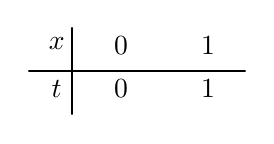
\begin{tikzpicture}[line cap=round,line join=round,>=triangle 45,x=1.10cm,y=1.10cm]
	\clip(0.48811571235680756,0.48483691302175425) rectangle (3.0081358090840915,1.5002103549181327);
	\draw (0.5,1.)-- (3.,1.);
	\draw (1.,1.5)-- (1.,0.5);
	\draw (0.6196407695972712,1.5002103549181327) node[anchor=north west] {$x$};
	\draw (0.6512067833349825,1.0004151374043713) node[anchor=north west] {$t$};
	\draw (1.3719640970127234,1.5107323594973698) node[anchor=north west] {$0$};
	\draw (2.376815534329866,1.5107323594973698) node[anchor=north west] {$1$};
	\draw (1.3719640970127234,1.0109371419836084) node[anchor=north west] {$0$};
	\draw (2.376815534329866,1.0109371419836084) node[anchor=north west] {$1$};
\end{tikzpicture}& \raisebox{-0.25cm}{\parbox[b]{5cm}{$$\Rightarrow I_2=\int_0^1 e^t\frac{dt}{2}=\frac{1}{2}\bigg.e^t\bigg|_0^1=\frac{1}{2}e-\frac{1}{2}$$}}
	\end{tabular}$$~\\[-10pt]
	Vậy $I=I_1+I_2=\dfrac{1}{3}+\dfrac{1}{2}e-\dfrac{1}{2}=\dfrac{1}{2}e-\dfrac{1}{6}$
\end{frame}

\begin{frame}{\textbf{\qquad Phân tích Đề thi THPT Quốc gia 2016}}~\\[-20pt]
	\cau{5}{Trong không gian $Oxyz$, cho 3 điểm $A(4;-4;3), B(1;3;-1),$ $C(-2;0;1)$. Viết phương trình mặt cầu $(S)$ đi qua các điểm $A, B, C$ và cắt hai mặt phẳng $(\alpha): \mbox{\textit{x}+\textit{y}+\textit{z}+2=0}$ và $(\beta): x-y-z-4=0$ theo hai giao tuyến là hai đường tròn có bán kính bằng nhau.}\pause
	Gọi $I(a;b;c)$ là tâm của mặt cầu $(S)$.
	Ta có hệ
	$$\begin{cases}
		IA=IB\\
		IA=IC\\
		d(I,(\alpha))=d(I,(\beta))
	\end{cases}\Leftrightarrow \begin{cases}
		a=1\\b=0\\c=3
	\end{cases}\vee \begin{cases}
		a=19/7\\
		b=-12/7\\
		c=-9/7
	\end{cases}$$~\\[-10pt]\pause
	\begin{itemize}[<+-|structure@+>]
		\item Với $(a;b;c)=(1;0;3)$, phương trình mặt cầu $$(x-1)^2+y^2+(z-3)^2=25$$
		
		
		\item  Với $(a;b;c)=(19/7;-12/7;-9/7)$, phương trình mặt cầu $$\left(x-\frac{19}{7}\right)^2+ \left(y+\frac{12}{7}\right)^2+ \left(z+\frac{9}{7}\right)^2=\frac{1237}{49}$$
	\end{itemize}
\end{frame}






\begin{frame}{\textbf{\qquad Phân tích Đề thi THPT Quốc gia 2016}}
	\cau{6}{\begin{enumerate}[a)]
			\item Viết phương trình tiếp tuyến của $(C)$ biết tiếp tuyến song song với đường thẳng $\Delta:$ $y=-x+1$
		\end{enumerate}}\pause
	Ta có 
	\begin{align*}
	&~(\sin x+\cos x)^2=1+\cos x\\
	\Leftrightarrow&~1+2\sin x\cos x=1+\cos x\\
	\Leftrightarrow&~\cos x\cdot(2\sin x-1)=0\\
	\Leftrightarrow&~\left[
	\begin{array}{l}
	\cos x=0\\[8pt]
	\sin x=\dfrac{1}{2}
	\end{array}
	\right.
	\Leftrightarrow \left[
	\begin{array}{l}
	x=\dfrac{\pi}{2}+k\pi\\[8pt]
	x=\dfrac{\pi}{6}+k2\pi\\[8pt]
	x=\dfrac{5\pi}{6}+k2\pi
	\end{array} (k\in\mathbb{Z})\right.
	\end{align*}
	Vậy phương trình đã cho có 3 họ nghiệm.
\end{frame}


\begin{frame}{\textbf{\qquad Phân tích Đề thi THPT Quốc gia 2016}}~\\[-18pt]
	\cau{6}{\begin{enumerate}[b)]
			\item Một tổ gồm 9 học sinh nam và 3 học sinh nữ. Cần chia tổ đó thành 3 nhóm, mỗi nhóm 4 học sinh để đi làm 3 công việc trực nhật khác nhau. Tính xác suất để khi chia ngẫu nhiên ta được mỗi nhóm có đúng 1 nữ.
		\end{enumerate}}\pause
	\begin{itemize}
		\item<+-|alert@+> Phép thử: ``Sắp 12 học sinh vào 3 nhóm khác nhau''\\[4pt]
		$\Rightarrow$ Số phần tử của không gian mẫu: $n(\Omega)=\C_{12}^4.\C^4_8.\C_4^4=34~ 650$\\[5pt]
		\item<+-|alert@+> Gọi $A$ là biến cố: ``Sắp 12 học sinh vào 3 nhóm \# có đúng 1 nữ''\\[4pt]
		$\Rightarrow$ Số kết quả thuận lợi cho biến cố $A$ là $$n(A)=\C_3^1.\C_9^3.\C_2^1.\C_6^3.\C^1_1.\C^3_3=10~080$$
		\item<+-|alert@+> Xác suất của biến cố là
		$P(A)=\dfrac{n(\Omega)}{n(A)}=\dfrac{10~080}{34~ 650}=\dfrac{16}{55}$\\
		\item<+-|alert@+> Vậy xác suất cần tìm là $\dfrac{16}{55}$
	\end{itemize}
\end{frame}


\begin{frame}{\textbf{\qquad Phân tích Đề thi THPT Quốc gia 2016}}~\\[-15pt]
	\Fontvi
	\cau{7}{Cho khối chóp $S.ABC$ có $SA\perp$ với mặt đáy $(ABC)$, tam giác $ABC$ vuông cân tại $B$, $SA=a$, $SB$ hợp với đáy một góc $30^0$. Tính thể tích của khối chóp $S.ABC$ và tính khoảng cách giữa $AB$ và $SC$.}\pause
	\divColSeven{
		\begin{center}
			\definecolor{uuuuuu}{rgb}{0.26666666666666666,0.26666666666666666,0.26666666666666666}
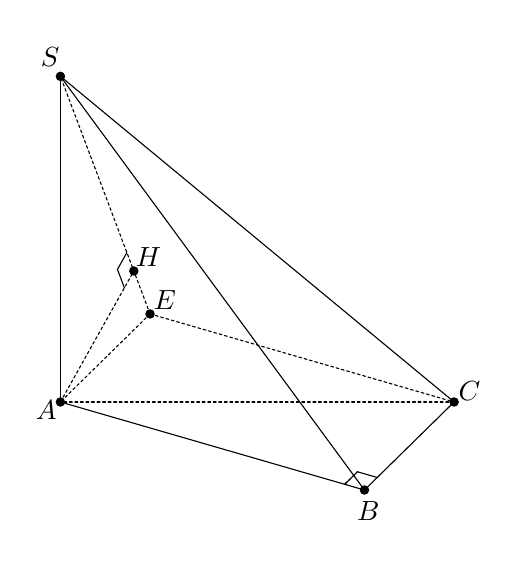
\begin{tikzpicture}[line cap=round,line join=round,>=triangle 45,x=1cm,y=1cm]
\clip(-0.41573723455466277,-1.6619803256614436) rectangle (5.456129498166213,4.7538066938798815);
\draw (0.,4.135715458856633)-- (0.,0.);
\draw [dash pattern=on 1pt off 1pt] (5.,0.)-- (0.,0.);
\draw (3.861454111806227,-1.1180600388409851)-- (0.,0.);
\draw (5.,0.)-- (3.861454111806227,-1.1180600388409851);
\draw (0.,4.135715458856633)-- (3.861454111806227,-1.1180600388409851);
\draw (0.,4.135715458856633)-- (5.,0.);
\draw [dash pattern=on 1pt off 1pt] (1.138545888193773,1.1180600388409851)-- (0.,4.135715458856633);
\draw [dash pattern=on 1pt off 1pt] (1.138545888193773,1.1180600388409851)-- (0.,0.);
\draw [dash pattern=on 1pt off 1pt] (1.138545888193773,1.1180600388409851)-- (5.,0.);
\draw [dash pattern=on 1pt off 1pt] (3.610224571325633,-1.0453180868056293)-- (3.772373824696389,-0.8860863839804118);
\draw (4.023603365176983,-0.9588283360157674)-- (3.772373824696389,-0.8860863839804118);
\draw (3.772373824696389,-0.8860863839804118)-- (3.610224571325633,-1.0453180868056293);
\draw [dash pattern=on 1pt off 1pt] (0.,0.)-- (0.9325224907594017,1.6641141139245692);
\draw (0.7243885130994864,1.683890471152824)-- (0.8443151197879425,1.8979030668842352);
\draw (0.7243885130994864,1.683890471152824)-- (0.8125958840709456,1.450101518193158);
\draw [fill=black] (0.,4.135715458856633) circle (1.5pt);
\draw[color=black] (-0.13030986404768772,4.382951952865932) node {$S$};
\draw [fill=black] (0.,0.) circle (1.5pt);
\draw[color=black] (-0.18086256524582772,-0.105495815799136106) node {$A$};
\draw [fill=black] (5.,0.) circle (1.5pt);
\draw[color=black] (5.196531179456448,0.14284608060644366) node {$C$};
\draw [fill=black] (3.861454111806227,-1.1180600388409851) circle (1.5pt);
\draw[color=black] (3.910901410608088,-1.3787637599470292) node {$B$};
\draw [fill=black] (1.138545888193773,1.1180600388409851) circle (1.5pt);
\draw[color=black] (1.3283854506071825,1.292495777749687) node {$E$};
\draw [fill=black] (0.9325224907594017,1.6641141139245692) circle (1.5pt);
\draw[color=black] (1.1182344306992774,1.8364160645701462) node {$H$};
\end{tikzpicture}
		\end{center}~\\[-20pt]
		\begin{itemize}
			\setlength{\itemindent}{-0.4cm}
			\item Ta có $SA\perp AB$
			\item $\Rightarrow AB$ là hình chiếu của $SB$ lên $(ABC)$, do đó $\widehat{SBA}=30^0$
			
		\end{itemize}\pause 
	}{
		\begin{itemize}
		    \setlength{\itemindent}{-0.5cm}
			\item $\cot \widehat{SBA}=\dfrac{AB}{SA} \Rightarrow BC=a\sqrt{3}$
			\item $S_{ABC}=\dfrac{1}{2}AB.BC=\dfrac{1}{2}a\sqrt{3}.a\sqrt{3}=\dfrac{3a^2}{2}$
			\item $V=\frac{1}{3}SA.S_{ABC}=\dfrac{1}{3}.a.\dfrac{3a^2}{2}=\dfrac{a^3}{2}$
			\item Trong mp$(ABC)$, kẻ $AI\parallelsum BC$ và kẻ $CI\parallelsum AB$\\
			$\Rightarrow ABCI$ là hình vuông cạnh $a\sqrt{3}$
			\item $d(AB,SC)=d\Big(A;(SIC)\Big)=AH$
			\item Tam giác $SAI$ vuông tại $A$ nên\\[-15pt] $$\frac{1}{AH^2}=\frac{1}{SA^2}+\frac{1}{AI^2}\Rightarrow AH=\frac{a\sqrt{3}}{2}$$~\\[-0.4cm]
			$\Rightarrow$ khoảng cách của $AB$ và $SC$ bằng $\dfrac{a\sqrt{3}}{2}$
		\end{itemize}
	}
\end{frame}



\begin{frame}{\textbf{\qquad Phân tích Đề thi THPT Quốc gia 2016}}~\\[-20pt]
	\Fontvi
	\cau{8}{Trong mặt phẳng tọa độ $Oxy$, cho hình chữ nhật $ABCD$ có hình chiếu $B$ lên $AC$ là $E(5;0)$, trung điểm $AE$ và $CD$ lần lượt là $F(0;2), I\left(\dfrac{3}{2};-\dfrac{3}{2}\right)$. Viết phương trình đường thẳng $CD$.}\pause
	\divColEight{
		\begin{center}
			\definecolor{uuuuuu}{rgb}{0.26666666666666666,0.26666666666666666,0.26666666666666666}
\begin{tikzpicture}[line cap=round,line join=round,>=triangle 45,x=0.38cm,y=0.38cm]
\clip(-5.9753393107991934,-2.9720284778930766) rectangle (9.357351755660217,6.118066940079262);
\draw (-5.,4.)-- (7.5,-1.);
\draw (0.,2.)-- (7.,5.);
\draw (0.3663874038598731,2.157023173082803)-- (0.5190246639022911,1.8008695663171608);
\draw (0.15263726004241795,1.643846393234358)-- (0.5190246639022911,1.8008695663171608);
\draw (5.141396521444867,0.35349130361216696)-- (5.513478835181248,0.20465837811761486);
\draw (5.372082313736382,-0.14883292549455263)-- (5.513478835181248,0.20465837811761486);
\draw (5.,0.)-- (7.,5.);
\draw (7.,5.)-- (7.5,-1.);
\draw (0.,2.)-- (1.5,-1.5);
\draw (-5.,4.)-- (-4.5,-2.);
\draw (-5.,4.)-- (7.,5.);
\draw (-4.5,-2.)-- (7.5,-1.);
\draw (7.,5.)-- (1.5,-1.5);
\draw [->] (-6.,0.) -- (9.,0.);
\draw [->] (0.,-3.) -- (0.,6.);
\draw (-0.8366698630922281,2.2118813588622332) node[anchor=north west] {\tiny 2};
\draw (-0.9826954922966035,0.1010351157088592) node[anchor=north west] {\scriptsize O};
\draw (4.501999584614738,0.01276293904934377) node[anchor=north west] {\tiny 5};
\draw (0.8791312800591822,0.9619295288777808) node[anchor=north west] {\tiny 1.5};
\draw (-1.6017339361031664,-0.8736952982362025) node[anchor=north west] {\tiny -1.5};
\draw [dash pattern=on 1pt off 1pt] (1.5,0.)-- (1.5,-1.5);
\draw [dash pattern=on 1pt off 1pt] (0.,-1.5)-- (1.5,-1.5);
\draw (8.09788070377248,1.09450973539879691) node[anchor=north west] {\scriptsize \textit{x}};
\draw (-1.1914294740438689,6.1545733473803566) node[anchor=north west] {\scriptsize \textit{y}};
\begin{scriptsize}
\draw [fill=black] (-5.,4.) circle (1.0pt);
\draw[color=black] (-5.4277432012827855,4.3657593896267635) node {$A$};
\draw [fill=black] (0.,2.) circle (1.0pt);
\draw[color=black] (0.40256734627472676,2.4579069880666084) node {$F$};
\draw [fill=black] (5.,0.) circle (1.0pt);
\draw[color=black] (4.794050843023488,0.5508398266624686) node {$E$};
\draw [fill=black] (1.5,-1.5) circle (1.0pt);
\draw[color=black] (1.5084741859250428,-1.9585830552097178) node {$I$};
\draw [fill=black] (7.,5.) circle (1.0pt);
\draw[color=black] (7.312992946798963,5.406191997707935) node {$B$};
\draw [fill=uuuuuu] (7.5,-1.) circle (1.0pt);
\draw[color=uuuuuu] (7.86058905631537,-1.2379741310911243) node {$C$};
\draw [fill=uuuuuu] (-4.5,-2.) circle (1.0pt);
\draw[color=uuuuuu] (-4.953159906368565,-2.3879259610755765) node {$M$};
\draw [fill=black] (0.,-1.5) circle (1.0pt);
\draw [fill=black] (1.5,0.) circle (1.0pt);
\draw [fill=black] (0.,0.021496920796609448) circle (1.0pt);
\end{scriptsize}
\end{tikzpicture}
		\end{center}~\\[-20pt]
		\begin{itemize}
			\setlength{\itemindent}{-0.4cm}
			\item $F$ là trung điểm $AE$ nên $A(-5;4)$
			\item Phương trình đường thẳng $(AC):$ $2x+5y-10=0$
		\end{itemize}\pause
	}{
	\begin{itemize}
		\setlength{\itemindent}{-0.2cm}
		\item Ta đi chứng minh: $BF\perp IF$.
		\item $\overrightarrow{BF}=\dfrac{1}{2}\left(\overrightarrow{BA}+ \overrightarrow{BE}\right)$\\[8pt]
		\item $\overrightarrow{FI}=\dfrac{1}{2}\left(\overrightarrow{FD}+\overrightarrow{FC}\right)=\dfrac{1}{2}\left(\overrightarrow{AD}+\overrightarrow{EC}\right)$
		\item $\Rightarrow \overrightarrow{BF}.\overrightarrow{FI}=0$
		\item $BF\perp IF$ nên có phương trình: $7x+3y-6=0$
		\item $BE$ đi qua $E$ và vuông góc $EF$ nên có phương trình: $5x-2y-25=0$.
		Do đó $B(7;5)$	
		\item Từ đây tìm được phương trình $(CD):$ $2x-24y-39=0$
	\end{itemize}
}
\end{frame}

\begin{frame}{\textbf{\qquad Phân tích Đề thi THPT Quốc gia 2016}}
	\Fontvi
	\cau{9}{Giải bất phương trình: \begin{equation}\label{eq_9}
			\left(2-\dfrac{3}{x}\right)\left(2\sqrt{x-1}-1\right) \geq \dfrac{4-8x+9x^2}{3x+2\sqrt{2x-1}}
		\end{equation}}\pause
	\begin{itemize}
		\item<+-|alert@+>  ĐK: $x\geq 1$. Ta có
		\begin{align}
			(\ref{eq_9})&\Leftrightarrow \frac{(2x-3)\left(2\sqrt{x-1}-1\right)}{x}\geq \frac{9x^2-4(2x-1)}{3x+2\sqrt{2\sqrt{2x-1}}}\nonumber\\
			&\Leftrightarrow \frac{(2x-3)\left(2\sqrt{x-1}-1\right)}{x}\geq 3x-2\sqrt{2x-1}\nonumber\\
			&\Leftrightarrow (2x-3)\left(2\sqrt{x-1}-1\right)\geq 3x^2-2x\sqrt{2x-1} \quad(\mbox{do }x\geq 1)\nonumber\\
			&\Leftrightarrow 2\left(x-1-\sqrt{x-1}\right)^2+\left(x-\sqrt{2x-1}\right)^2+2\left(\sqrt{x-1}+x-1\right)\leq 0\label{ptcau9_2}
		\end{align}
		\item<+-|alert@+> $\Rightarrow \mbox{VT}_{(\ref{ptcau9_2})}\geq 0$
		\item<+-|alert@+> Vậy để $(\ref{ptcau9_2})$ xảy ra thì $\Leftrightarrow \mbox{VT}_{(\ref{ptcau9_2})}=0\Leftrightarrow
		\begin{cases}
		x-1=\sqrt{x-1}\\[6pt]
		x=\sqrt{2x-1}\\[6pt]
		x-1=0
		\end{cases}\Leftrightarrow x=1$
	\end{itemize}
\end{frame}


\begin{frame}{\textbf{\qquad Phân tích Đề thi THPT Quốc gia 2016}}~\\[-18pt]
	\FontviTen
	\cau{10}{Cho $a, b, c>0$, thỏa $c=\min\{a,b,c\}$. Tìm giá trị nhỏ nhất của biểu thức\\[-2pt]
		\begin{equation}\label{eq_pt10}
			P=\sqrt{\dfrac{a}{b+c}}+\sqrt{\dfrac{b}{c+a}}+\dfrac{2\ln\left( \dfrac{6(a+b)+4c}{a+b}\right)}{\sqrt[4]{\dfrac{8c}{a+b}}}
		\end{equation}}\pause
	\begin{itemize}
		\item ~\\[-24pt]
		\begin{align}
			\sqrt{\frac{a}{b+c}}+\sqrt{\frac{b}{c+a}}=\frac{a^2}{a\sqrt{a(b+c)}} +\frac{b^2}{b\sqrt{b(c+a)}}&\geq \frac{(a+b)^2}{a\sqrt{a(b+c)}+ b\sqrt{b(c+a)}}\label{eq10_1}
		\end{align}
		\item Mặt khác, vì $c=\min \{a,b,c\}\Rightarrow a+b-2c\geq 0$. Nên ta có
		$$a^2(b+c)+b^2(c+a)=ab(a+b-2c)+c(a+b)^2\leq \left(\frac{a+b}{2}\right)^2(a+b-2c)+c(a+b)^2$$
		\begin{equation}\label{eq10_2}
			\left(\frac{a+b}{2}\right)^2(a+b-2c)+c(a+b)^2=\frac{(a+b)^3+2c(a+b)^2}{4}
		\end{equation}
		\item Từ $(\ref{eq10_1})$ và $(\ref{eq10_2})$ suy ra $\sqrt{\dfrac{a}{b+c}}+\sqrt{\dfrac{b}{c+a}}\geq 2\sqrt{\dfrac{a+b}{a+b+2c}}$\\[12pt]
		\item ~\\[-27pt]
		\begin{equation}\label{eq10_3}
		\ln\left[\frac{6(a+b)+4c}{a+b}\right]=\ln\left[2\left(\frac{a+b+2c}{a+b}+2\right)\right]\geq \ln\left[\left(\sqrt{1+\frac{2c}{a+b}}+\sqrt{2}\right)^2\right]
		\end{equation}
	\end{itemize}
\end{frame}

\begin{frame}{\textbf{\qquad Phân tích Đề thi THPT Quốc gia 2016}}
	\FontviTen
	\begin{itemize}[<+-|structure@+>]
		\item Mặt khác: vì $c=\min\{a,b,c\}\Rightarrow 2c\leq a+b$. Nên ta có
		\begin{equation}\label{eq10_4}
		\sqrt[4]{\frac{8c}{a+b}}\leq \sqrt[4]{2\cdot\frac{a+b+2c}{a+b}}\leq\frac{1}{2} \left(\sqrt{1+\frac{2c}{a+b}}+\sqrt{2}\right)
		\end{equation}
		\item Từ $(\ref{eq10_2}), (\ref{eq10_3}), (\ref{eq10_4})$ ta được\\[-15pt]
		$$P\geq \frac{2}{\sqrt{1+\dfrac{2c}{a+b}}}+\frac{8\ln\left( \sqrt{1+\dfrac{2c}{a+b}}+\sqrt{2}\right)}{\sqrt{1+\dfrac{2c}{a+b}}+\sqrt{2}}$$
		\item Đặt $t=\sqrt{1+\dfrac{2c}{a+b}}$, do $c=\min\{a,b,c\}\Rightarrow \dfrac{2c}{a+b}\leq 1\Rightarrow t\leq \sqrt{2}$\\[10pt]
		\item Xét hàm $f(t)=\dfrac{2}{t}+\dfrac{8\ln\left(t+\sqrt{2}\right)}{t+\sqrt{2}}$, trên $t\in\left(0;\sqrt{2}\right]$\\[10pt]
		\item Ta có
		$$f'(t)=
		\frac{\left(t-\sqrt{2}\right)\left(3t+\sqrt{2}\right)}{t^2\left(t+\sqrt{2}\right)^2}-\frac{8\ln\left(t+ \sqrt{2}\right)}{\left(t+\sqrt{2}\right)^2},~\forall t\in\left(0;\sqrt{2}\right] 
		$$
		\item Suy ra: $f(t)\geq f(\sqrt{2})=2\left(1+\ln 8\right)$. Vậy $P_{\min} =2\left(1+\ln 8\right)$.\\[8pt]
		Dấu ``$=$'' xảy ra khi và chỉ khi $a=b=c$.
	\end{itemize}
\end{frame}




















\end{document} 
